\section{Face authentication}
    Face recognition is a problem that has been around for a while and
    human-level solutions have been developed, such as FaceNet\cite{arXiv:1503.03832}.
    However, there are many subtleties to face recognition in mobile devices
    security, in particular when using unconventional cameras.

    From the security context, false positives are very problematic. This observation alone
    poses two questions:
    \begin{itemize}
      \item How to measure a model's performance to punish false positives?
      \item How to maximize our chosen score measure?
    \end{itemize}
    We have tackled two problems in our research -- multi-class and binary classification.
    Binary classification is more adequate to the possible applications of our research.
    Multi-class classification allows the reader to compare the achieved results
    with other face recognition models.

    The second observation is more optimistic: the front camera of a mobile is capable of
    capturing relatively many frames per second. We decided not to constrain our
    methods to a classification based on a single frame.
    Moreover, a large training set can be built
    when adding a new user to the device -- it is not unreasonable to make that procedure
    longer for increased security. We aimed to take advantage of those factors.

    \subsection{Data set}
    We have set requirements for our dataset, aiming to reflect real-life
    appliances:
    \begin{itemize}
        \item \textbf{depth and IR channels}: in real-life appliance, leveraging
        the infrared camera allows equally good vision regardless of lighting
        conditions.
        \item \textbf{various vertical angles}: when a user is looking at their
        mobile device,
        their head may be placed at various angles along the vertical axis.
        However, it is reasonable to assume that the angle along the horizontal
        axis will be small, especially if the user is consciously trying to
        unlock the device.
        \item \textbf{many frames per subject}: when a new user is being added
        to a mobile device's authentication system, it is acceptable to require
        them to look at the camera, at various angles, for a short period of
        time. Many frames can (and should) be taken.
    \end{itemize}

    There are several good databases for face recognition with depth camera:
    The EURECOM Kinect Face Database\cite{eurecom},
    RGB-D Face database \cite{vapaaudk},
    The Florence Superface dataset\cite{superface}. However, none of them was
    deemed suiting for our project, primarily due to the lack of IR channel.
    Thus, we have decided to build a dedicated dataset.

    \subsubsection*{Data collection}
    The dataset consists of $44$ subjects: $36$ males and
    $8$ females, mostly aged $20$-$25$. Each subject has been asked to
    follow an object with their entire head, making two cycles of slow,
    continuous movements: \texttt{up $\to$ center $\to$ down $\to$ center $\to$
    left $\to$ center $\to$ right $\to$ center}.
    That procedure has resulted in approximately $20$ seconds of footage per
    subject.

    IR and depth frames are synchronized, taken at $10$ FPS rate.

    Dataset contains also RGB frames taken at $10$ FPS rate, not synchronized
    with IR and depth frames.

    The procedure performed to collect photos of a single person took around $20$-$30$ seconds.
    We believe it could be proposed as a part of mobile device's first time security configuration.

    \subsubsection*{Test set}
    For the test set, we have chosen approximately first $25\%$ of
    frames from each subject -- the first two vertical head rotations.

    \subsubsection*{Samples}
    \begin{figure}[H]
    \caption{One of the subjects from the database -- the first $269$ IR frames.}
    \centering
    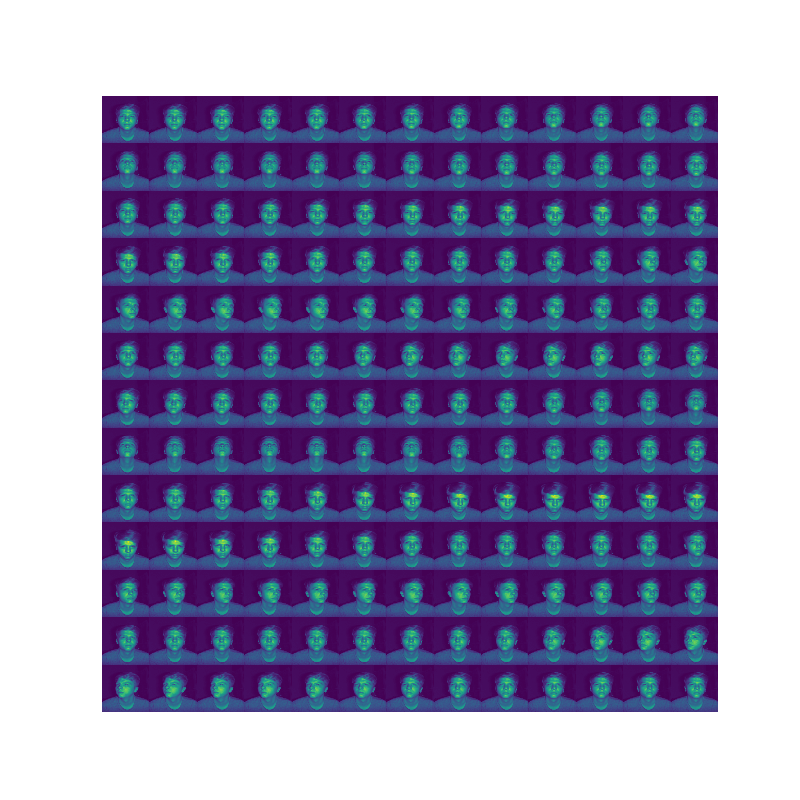
\includegraphics[scale=0.5]{tiled_faces_ludziej}
    \end{figure}

    \subsection{Face angle detection}
    \label{sec:angledetection}
    Longer description of angle detection

    \subsection{Normalization}
        \subsubsection*{Depth mean and standard deviation normalization}
        Let $F$ be the set of all points belonging to the trimmed face and
        $d(p)$ -- depth of the point $p$. Let $\mu$ denote the mean depth, i.e.
        $\mu = \frac{\sum\limits_{p \in F}{d(p)}}{|F|}$ and $\sigma$ -- standard
        deviation, i.e. $\sigma = \sqrt{\frac{1}{|F|} \sum\limits_{p \in F}{(d(p) - \mu)^2}}$.
        For each pixel $p$, its new depth is calculated as:

        \begin{center}
        $
          d'(p) = \begin{cases}
                  d(p) - \mu &\quad\text{if}\ |d(p) - \mu| \leqslant 2 \cdot \sigma \\
                  0 &\quad\text{otherwise}
                  \end{cases}
        $
        \end{center}


        Lastly, all depth values are scaled to the interval $[0..1]$:
        \begin{center}
        $
          d''(p) = \frac{d'(p) - min(\{d'(r)\ |\ r \in F\})}{max(\{d'(r)\ |\ r \in F\}) - min(\{d'(r)\ |\ r \in F\})}
        $
        \end{center}

        \subsubsection*{Face angle normalization}
        Depth channel provides substantial information about faces' geometry, thus allowing
        a meaningful normalization method -- rotation to the frontal position.

        With our ability to detect face angle (\ref{sec:angledetection}), we can obtain
        three values: $\theta_x, \theta_y, \theta_z$ -- angles along each axis.

        The face can be represented as a cloud of $3$-dimensional, "colorful" points.
        Point $p$ is defined as a vector $[x_p, y_p, z_p, ir_p]^{T}$.

        Let $R_x(\theta_x), R_y(\theta_y), R_z(\theta_z)$ denote the rotation matrices
        for $X, Y, Z$ axes, as follows:
        \[
        R_x(\theta_x) =
        \begin{bmatrix}
        1 & 0 & 0\\
        0 & cos(\theta_x) & -sin(\theta_x)\\
        0 & sin(\theta_x) & cos(\theta_x)
        \end{bmatrix}
        \]
        \[
        R_y(\theta_y) =
        \begin{bmatrix}
        cos(\theta_y) & 0 & sin(\theta_y)\\
        0 & 1 & 0\\
        -sin(\theta_y) & 0 & cos(\theta_y)
        \end{bmatrix}
        \]
        \[
        R_z(\theta_z) =
        \begin{bmatrix}
        cos(\theta_z) & -sin(\theta_z) & 0\\
        sin(\theta_z) & cos(\theta_z) & 0\\
        0 & 0 & 1
        \end{bmatrix}
        \]
        The operation of rotating a single point is a product of its coordinates and the three rotation matrices:
        \begin{center}
        $
        \begin{bmatrix}
          x_p\\
          y_p\\
          z_p\\
          ir_p
        \end{bmatrix}
        \cdot
        \begin{bmatrix}
          R_x & 0_{3}^T\\
          0_{3} & 1
        \end{bmatrix}
        \cdot
        \begin{bmatrix}
          R_y & 0_{3}^T\\
          0_{3} & 1
        \end{bmatrix}
        \cdot
        \begin{bmatrix}
          R_z & 0_{3}^T\\
          0_{3} & 1
        \end{bmatrix}
        $
        \end{center}


    \subsection{Preprocessing techniques}
    We have tried several different preprocessing techniques.
        \subsubsection*{Trimming faces}
        During the process of collecting the dataset, each subject has been
        recorded in only one set of clothes (the ones they were wearing at the
        time), one hairstyle and the background may slightly vary among the
        subjects (the background behind subjects recorded at $12$ a.m. is
        likely to be brighter than behind the subjects recorded at $4$ p.m.).

        Since a classifier might leverage those factors, photos have been
        trimmed to polygons containing the faces. Such polygons have been
        found with Face Recognition library \cite{facerecog} on IR photos.
        Depth photos have been trimmed accordingly.

        \begin{figure}[H]
        \caption{Before and after trimming the face.}
        \centering
        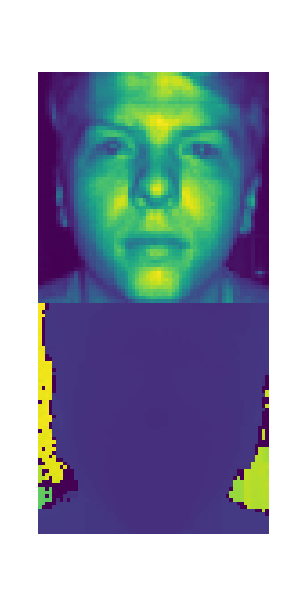
\includegraphics[scale=0.25]{before_trim_ludziej}
        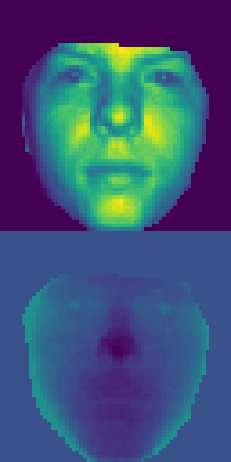
\includegraphics[scale=0.25]{after_trim_ludziej}
        \end{figure}

        \subsubsection*{Entropy maps}
        How they work, why to use them (reference to the other paper).

        \subsubsection*{HOGs of entropy maps}
        How they work, why to use them (reference to the other paper). They
        are particularly helpful for Extra Trees and RDF-s.

        \subsubsection*{Channels vs concatenation}
        A choice of the input format passed to a classifier is not only a matter
        of images to include. Another decision to be made is whether different
        channels (IR, depth) and different preprocessed images (entropy maps,
        HOGs) should be concatenated or layered as channels. In our experiments,
        we have included both approaches.

        \subsubsection*{Data augmentation}
        To further enhance the training set, we have used image augmentations, with \texttt{imgaug}\cite{imgaug} library.
        The used transformations include:
        \begin{itemize}
            \item \textbf{coarse salt and pepper} -- randomly placed patches of grain (black and white pixels)
            \item \textbf{padding} -- shifting the input image $3$ pixels in random direction
            \item \textbf{Gaussian blur} with several different strenghts
            \item \textbf{rotations} by $2$ degrees
            \item \textbf{PiecewiseAffine} -- augmenter that places a regular grid of points on an image and randomly moves the neighbourhood of these point around via affine transformations.
        \end{itemize}
        \begin{figure}[H]
        \caption{Trimming + all possible augmentations.}
        \centering
        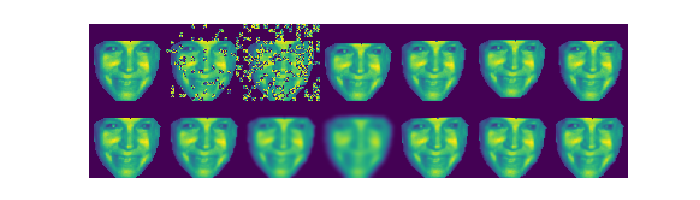
\includegraphics[scale=0.5]{augmenters}
        \end{figure}

    \subsection{Classifiers}
        \subsubsection{Convolutional Neural Network}
        We have used a convolutional neural network with the following structure:
        \begin{itemize}
            \item \textbf{Layers}:
            \begin{itemize}
            \item[$\blacksquare$] \textbf{conv. layer 0}: $20$ filters, $5 \text{x} 5$ kernel
            \item[$\blacksquare$] \textbf{max pooling}: $2 \text{x} 2$ pool size, $2 \text{x} 2$ strides
            \item[$\blacksquare$] \textbf{conv. layer 1}: $20$ filters, $5 \text{x} 5$ kernel
            \item[$\blacksquare$] \textbf{max pooling}: $2 \text{x} 2$ pool size, $2 \text{x} 2$ strides
            \item[$\blacksquare$] \textbf{conv. layer 2}: $40$ filters, $5 \text{x} 5$ kernel
            \item[$\blacksquare$] \textbf{max pooling}: $2 \text{x} 2$ pool size, $2 \text{x} 2$ strides
            \item[$\blacksquare$] \textbf{dense layer} with sigmoid activation function
            \end{itemize}
            \item \textbf{Loss function}: Log Loss
            \item \textbf{Optimizer}: SGD
            \item \textbf{Kernels initialization}: Since we have experimented with deeper
            networks too, and each model was trained from scratch, a reckless initialization
            would hamper the models ability to learn and increase the number of
            iterations needed for convergence. To ensure quick start of the learning
            process, we decided to initialize each kernel with \textbf{random normal
            distribution with $\mu = 0,\ \sigma = \sqrt{(2 / N)}$}, as advised by
            \citeauthor{initialization}.
        \end{itemize}


        \begin{figure}[H]
        \caption{Convolved input images (only IR channel). First two rows
        are outputs from first and second convolutional layers. Third and fourth
        row are outputs from all $40$ filters from last convolutional layer.
        }
        \centering
        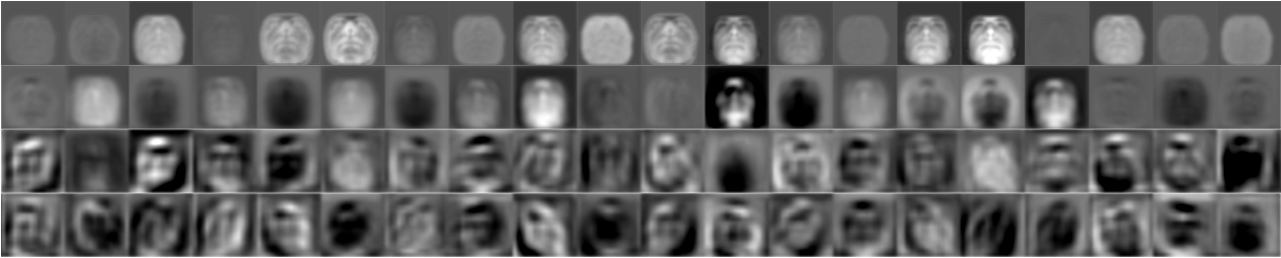
\includegraphics[scale=0.25]{convolutions}
        \end{figure}
        \begin{figure}[H]
            \caption{For each filter in each convolutional layer, $10$ patches
            among one of the test batches were chosen that activate those
            filters the most.
            Horizontally, consecutive filters are presented, vertically -- patches
            sorted from the highest activation.
            Note that from each patch, only IR channel is presented.
            }
            \centering
            \begin{subfigure}[b]{0.4\textwidth}
                \centering
                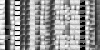
\includegraphics[scale=1.4]{exciting_layer0}
                \caption{conv. layer 0}
            \end{subfigure}
            \begin{subfigure}[b]{0.4\textwidth}
                \centering
                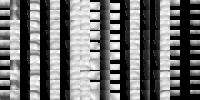
\includegraphics[scale=0.7]{exciting_layer1}
                \caption{conv. layer 1}
            \end{subfigure}
            \\
            \begin{subfigure}[b]{0.8\textwidth}
                \centering
                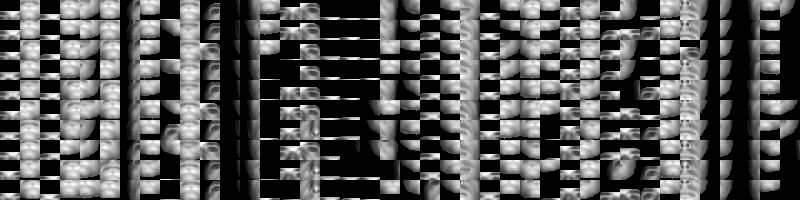
\includegraphics[scale=0.35]{exciting_layer2}
                \caption{conv. layer 2}
            \end{subfigure}
        \end{figure}

        \subsection{Ensembled SVMs and Extra Trees}

        \subsection{Ensembled CNN, SVMs and Extra Trees}

    \subsection{Quality measures}
        Models have been trained in two modes: multi-class and binary
        classification. Let $T$ be the test set, $p_t$ -- predictions for test input
        $t \in T$ and $y_t$ -- ground truth for test input $t \in T$.
        \subsubsection*{Accuracy}
        For classifiers trained in multi-class mode the accuracy score has been
        measured:

        \begin{center}
        $acc(p, y) = \frac{|\{t \in T\ |\ p_t = y_t\}|}{|T|}$
        \end{center}

        \subsubsection*{Recall for fixed precision}

        When testing the model in binary mode two decisions are being made:
        \begin{itemize}
            \item \textbf{positive class (device owner)}: One subject from the
            database is chosen as the "device owner". All photos of this subjects
            are then labeled as positive. All photos of other subjects are
            labeled as negative.
            \item \textbf{desired precision threshold:}
            Precision is defined as:
            \begin{center}
            $prec(p, y) = \frac{\{t \in T\ |\ y_t = p_t = 1\}}{\{t \in T\ |\ p_t = 1\}}$
            \end{center}
            We have chosen $3$ different precision thresholds: $0.99$, $0.995$, $0.999$.
        \end{itemize}
        Recall is defined as:
        \begin{center}
        $rec(p, y) = \frac{\{t \in T\ |\ p_t = y_t = 1\}}{\{t \in T\ |\ y_t = 1\}}$
        \end{center}
        For each precision threshold, we have calculated the corresponding recall measure and
        averaged the result over $5$ random choices for positive class.

    \begin{figure}[H]
    \caption{Test samples misclassified by CNN}
    \centering
    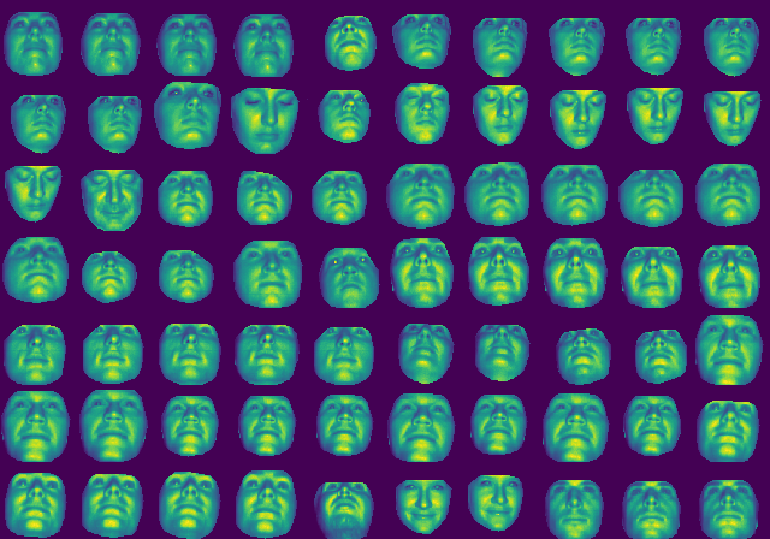
\includegraphics[scale=0.4]{misclassified}
    \end{figure}


    \subsection{Single-frame model results}
        We call a model single-frame if it classifies the person on the photo
        using only one frame. We have evaluated several single-frame model to
        choose one multi-class and one binary classifier.
        \subsubsection{Multi-class}
        \begin{center}
        \begin{tabular}{ |c|c|c|c|c| }
            \hline
            Model & Entropy & HOGs & CNN inputs & Accuracy\\
            \hline
            CNN & y & n & channels & 0.9721\\
            \hline
            CNN 10 : 1 SVM & y & y & channels & 0.9721\\
            \hline
            CNN 1 : 2 SVM & y & y & channels & 0.9536\\
            \hline
            SVM & n & y & channels & 0.9099\\
            \hline
            SVM 1:10 ET & n & y & channels & 0.8884\\
            \hline
            ET & n & y & channels & 0.8369\\
            \hline
        \end{tabular}
        \end{center}

        \subsubsection{Binary}
        \begin{center}
        \begin{tabular}{ |c|c|c|c|c|c|c| }
            \hline
            \multirow{2}{*}{Model} &
            \multirow{2}{*}{Entropy} &
            \multirow{2}{*}{HOGs} &
            \multirow{2}{*}{CNN inputs} &
            \multicolumn{3}{|c|}{Recall for precision $\rho$} \\
            & & & & $\rho = 0.99$ & $\rho = 0.995$ & $\rho = 0.999$ \\
        \hline
        CNN 1 : 5 SVM & y & y & channels & 0.9013 & 0.8947 & 0.8947 \\
        \hline
        CNN & y & y & channels & 0.8487 & 0.8487 & 0.8487 \\
        \hline
        \end{tabular}
        \end{center}

    \subsection{Multiple frames based classification}

    \subsection{Proposed solution}
